\section{Learning to describe new objects from corpora}
\label{sec:learning}

In the previous section we presented an algorithm that assumes that each relation R 
used in a referring expression has a known probability of use R.\puse. 
Intuitively, the R.\puse~is the probability of using relation R to describe the target. In Tables~\ref{probability-of-use} and~\ref{probability-of-use-people} we show the probabilities of use that we are able to learn from corpora and to apply to the models of Figures~\ref{Tuna-scene} and \ref{Tuna-people-scene}.  In Figure~\ref{Tuna-scene}, the probability of using \emph{blue} to describe the target is higher than the probability of using \emph{facing left}, although both are properties of the target.

The probability of using green is not cero because a green object may be used in a relational description of the target (for example, ``the blue chair far from the green fan''). 

In this section, we describe how to calculate these probabilities from corpora.  
The general set up is the following: we assume available a corpus of REs associated 
to different scenes that are prototypical of the domain in which the GRE algorithm has to operate; we call this, the training data.   
We then show how to generalize these values to other scenes in the domain, using a machine learning algorithm. We exemplify the methodology using the TUNA corpus. 

\begin{table}[h!]
 \begin{minipage}{0.48\textwidth} 
%\begin{center}
\begin{tabular}{|l|c|}
\hline
Top 10 relations in Figure \ref{Tuna-scene} & learned \puse\\
\hline
chair 	&	0.94	\\
blue 	&	0.89	\\
y3 	&	0.29	\\
x5 	&	0.27	\\
left 	&	0.25	\\
large 	&	0.21	\\
green 	&	0.05	\\
small 	&	0.05	\\
back 	&	0.02	\\
y1 	&	0.02	\\
\hline
\end{tabular}
%\vspace*{.09cm}
\caption{Probabilities of use learned from corpora and instantiated for Figure~\ref{Tuna-scene}} 
\label{probability-of-use}
%\end{center}
\end{minipage}
\begin{minipage}{0.48\textwidth} 
%\begin{center}
\begin{tabular}{|l|c|}
\hline
Top 10 relations in Figure \ref{Tuna-people-scene} & learned \puse\\
\hline
person 	&	0.79	\\
hasGlasses 	&	0.71	\\
y2 	&	0.20	\\
x5 	&	0.18	\\
hasHair	&	0.13	\\
hairDark 	&	0.13	\\
hairLight 	&	0.11	\\
ageOld 	&	0.05	\\
y3 	&	0.03	\\
x2 	&	0.02	\\
\hline 
\end{tabular}
%\begin{center}
%\vspace*{.09cm}
\caption{Probabilities of use learned from corpora and instantiated for Figure~\ref{Tuna-people-scene}} 
\label{probability-of-use-people}
%\end{center}
\end{minipage}
\end{table}
%\vspace*{-.9cm}
%\end{table}


\label{tunaDescription}The TUNA Corpus~\cite{gatt-balz-kow:2008:ENLG} is a set of human-produced referring expressions (REs) for entities in visual domains of pictures of furniture and people as exemplified in Figures~\ref{Tuna-scene} and~\ref{Tuna-people-scene}. The corpus was
collected during an online elicitation experiment in which subjects typed descriptions of a target single referent or pair of referents. 
In each picture there were 5 or 6 other objects. 
In the experiment, the participation was not controlled, but there was a main condition manipulated the +/-LOC: in +LOC condition, participants were told that they could refer to entities using any of their properties (including their location on the screen). In the -LOC condition, they were discouraged from doing so, though not prevented. 
The attributes for each entity include properties such as an object's color or a person's characteristic such as having dark hear.
In this paper we will use the singular part of the TUNA corpus. The corpus contains 780 singular referring expressions divided
into 80\% training data, 20\% test. 

%XML Format Guidelines for the TUNA Corpus dice 	
In order to collect the corpus, each participant in the elicitation experiment carried out 38 trials, 20 furniture descriptions and 18 people descriptions.  
%http://staff.um.edu.mt/albert.gatt/pubs/tunaFormat.pdf

%The furniture sub-corpus consists of 900 descriptions from 45 native or fluent speakers of English.
%Participants described objects in 20 trials (Evaluating algorithms for the Generation of Referring Expressions
%using a balanced corpus)

\begin{figure}[ht]
%\begin{minipage}{0.60\linewidth}
\centering
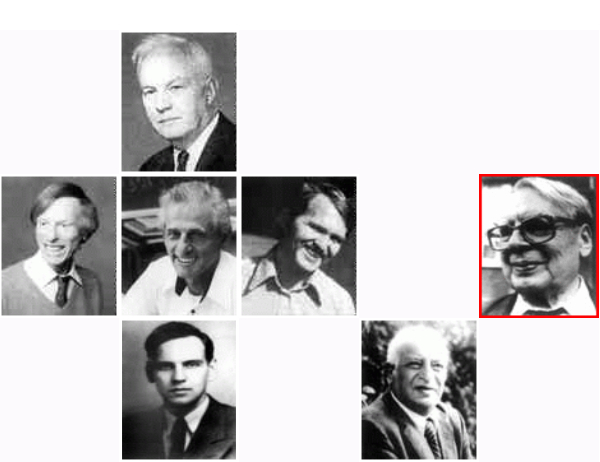
\includegraphics[width=0.8\textwidth]{images/tuna-people.jpg}

%\vspace*{-.4cm}
\caption{Scene used during the collection of the TUNA corpus. The referring expression collected has to distinguish the target from the rest of the people. For this scene, the RE was \emph{the man with glasses}}. 
\label{Tuna-people-scene}
%\end{minipage}
%\vspace*{-.38cm}
%\begin{minipage}{0.50\linewidth}
\centering
%\vspace*{.2cm}
%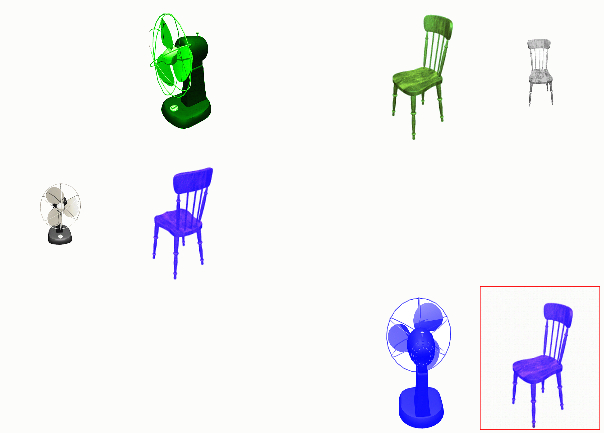
\includegraphics[width=\textwidth]{images/tuna.jpg}
%\vspace*{-.25cm}
%\vspace*{-.4cm}

%\caption{TUNA corpus furniture scene}
%\label{Tuna-furniture-scene}
%\end{minipage}
\end{figure}

The TUNA corpus has two different domains called furniture and people. For each word in each domain we train a machine learning model that computes a function of its \puse. When this function is instantiated with a set of domain independent features that we define below. 

%The annotation of the TUNA corpus have just properties for objects and have not relations between them annotated, there is a relation given by the positions but is it not annotated as relational properties between objects.

%Suppose we want to automatically generate REs for target $t$ in a given scene, and that we do have available a corpus $C$ for scenes similar of REs in the same domain (this is exactly the kind of information we find in the TUNA corpus).  
%We use the models provided by TUNA as input of our algorithm.  
%We aisle the scene for which we want to compute the \puse\ and use all another REs of scenes. Then we estimate the value of \puse\ for each of the relations in the model as the percentage of REs 
%in which the relation appears. I.e., 
%\begin{equation}\label{eq1}
%R.\puse = \frac{\# \mbox{ of REs in $C$ in which R appears}}{\# \mbox{ of REs in $C$}}.
%\end{equation}

%\noindent
%This estimation is overly simplified and, for example, it does not differentiate between the properties of a target and the 
%properties of a landmark object used in a relational RE to complete the description of the target, but in this case people don't use too much descriptions of lansmarks. It is extremely easy 
%to compute, and we will see in Section~\ref{sec:evaluation} that it already produces natural REs that match those found in the corpus. 

To clarify the computation of R.\puse\ in the training data and the model $\gM$ associated to each scene we list the required steps in detail, 
and discuss how we carried them out in the TUNA corpus:

\begin{enumerate}
\item Tokenize the referring expressions and call the set of tokens $T$. In particular, multi-word expressions like ``in the top row'' 
should be matched to a single token like \emph{y1}.

\item Replace hyperonyms from $T$. E.g., if both \emph{man} and \emph{picture} appear in $T$, delete \emph{picture}.

\item If the set of tokens obtained in the previous steps contains synonyms normalize them to a representative in the synonym class, 
and call the resulting set $\REL$; it will be the signature of the model $\gM$ used by the algorithm. E.g., the tokens \emph{man} 
and \emph{guy} are both represented by the token \emph{man}.

\item For each scene, define $\gM$ such that the interpretation $\interp{\cdot}$ ensures that the RE of the scene in the corpus uniquely identifies the target in the model. E.g., the $\el$ formula $\exists$\emph{left}.$\top \sqcap \exists$\emph{blue}.$\top \sqcap \exists$\emph{chair}.$\top$, which represents the RE ``the blue chair facing left'' found in the corpus for this scene, denotes the target and only the target in the model $\gM$ depicted in Figure~\ref{TUNA-scene-graph}. If the corpus includes more than one RE per scene, the model should include all the properties used to describe the scene.

\item For each R $\in \REL$ we assign 1 to R.\puse\ if R occurs in the RE, we assign 0 otherwise. In case that the corpus has more than one RE per scene we calculate the proportion of appearance of each property.

\end{enumerate}


%For that reason, for example, the value of \emph{chair}.\puse\ is (AGREGAR ACA), while the value of \emph{fan}.\puse\ is (AGREGAR ACA)  
%These probabilities will not be useful to describe different targets in different scenes. We will see how we can use them to obtain
% values for new targets and scenes using a machine learning approach in the next section. Not surprisingly, using these values for 
%R.\puse\ the REs generated most often by the algorithm can be found in the corpus. More interestingly, as we discuss in 
%Section~\ref{sec:evaluation} the algorithm generates REs with a distribution that matches the one found in the corpus and, 
%as Table~\ref{results-algo-fig3} shows, even the generated REs not found in the corpus are natural.    


The learning was done with the machine learning toolkit WEKA~\cite{Hall:WEK09}, training on the training data of the TUNA corpus. We use linear regression to learn the function of \puse\ for each relation in the signature. 
For a given scene, we replace the variables of the obtained function by the values of the features in the scene that we want to describe. 
We use simple features to obtain the function, all the features can be extracted automatically from the relational model and are listed 
in Table~\ref{features}.  
%\vspace*{-.3cm}
\begin{table}[htbp]
\begin{center}
\begin{tabular}{|l|p{10cm}|}
\hline
target-has & whether the target element has the property \\
location-has & whether the RE may use the location of the target in the figure\\
discrimination & 1 over the number of objects in the model that have the property \\
\puse (learned) & probability of using the property to describe the target \\
\hline
\end{tabular}
\vspace*{.03cm}
\caption{Features used for learning the \puse~for each token in the signature of the scenes of the TUNA corpus} 
\label{features}
\end{center}
\end{table}
%\vspace*{-.9cm}
Our feature set is intentionally simplistic in order for it to be domain independent. As a result there are some complex relations 
between characteristics of the scenes that it is not able to capture. 

Starting from the scene in Figure~\ref{Tuna-scene}
the resulting signature and their associated \puse\ are listed in the Table~\ref{probability-of-use} and for the Figure~\ref{Tuna-people-scene} in Table~\ref{probability-of-use-people}. 

Notice that the values R.\puse\ obtained in this way should be interpreted as the probability of using R to describe the target in model 
$\gM$, and we could argue that they are correlated to the \emph{saliency} of R in the model.  

Using linear regression we are able to learn interesting characteristics of the domain. To start with, it learns known facts such that the 
saliency of a color depends strongly on whether the target object is of that color, and it does not depend on its discrimination power 
in the model. Moreover, it learns that size relations (e.g., large and small) is used more frequently when it has a higher discriminative power
which confirms a previous finding reported in~\cite{viet:gene11}. Finally, it is able to learn that the orientation properties (e.g., left and right) are used as a last resource, when it is necessary to identify the target uniquely in cases they were warned do not tu use the location of the object in the scene as explain in~\ref{tunaDescription}. 

